%%%%%%%%%%%%%%%%%%%%%%%%%%%%%%%%%%%%%%%%%
% Beamer Presentation
% LaTeX Template
% Version 1.0 (10/11/12)
%
% This template has been downloaded from:
% http://www.LaTeXTemplates.com
%
% License:
% CC BY-NC-SA 3.0 (http://creativecommons.org/licenses/by-nc-sa/3.0/)
%
%%%%%%%%%%%%%%%%%%%%%%%%%%%%%%%%%%%%%%%%%

%----------------------------------------------------------------------------------------
%	PACKAGES AND THEMES
%----------------------------------------------------------------------------------------

\documentclass{beamer}

\mode<presentation> {

% The Beamer class comes with a number of default slide themes
% which change the colors and layouts of slides. Below this is a list
% of all the themes, uncomment each in turn to see what they look like.

%\usetheme{default}
%\usetheme{AnnArbor}
%\usetheme{Antibes}
%\usetheme{Bergen}
%\usetheme{Berkeley}
%\usetheme{Berlin}
%\usetheme{Boadilla}
%\usetheme{CambridgeUS}
%\usetheme{Copenhagen}
%\usetheme{Darmstadt}
%\usetheme{Dresden}
%\usetheme{Frankfurt}
%\usetheme{Goettingen}
%\usetheme{Hannover}
%\usetheme{Ilmenau}
%\usetheme{JuanLesPins}
%\usetheme{Luebeck}
\usetheme{Madrid}
%\usetheme{Malmoe}
%\usetheme{Marburg}
%\usetheme{Montpellier}
%\usetheme{PaloAlto}
%\usetheme{Pittsburgh}
%\usetheme{Rochester}
%\usetheme{Singapore}
%\usetheme{Szeged}
%\usetheme{Warsaw}

% As well as themes, the Beamer class has a number of color themes
% for any slide theme. Uncomment each of these in turn to see how it
% changes the colors of your current slide theme.

%\usecolortheme{albatross}
%\usecolortheme{beaver}
%\usecolortheme{beetle}
%\usecolortheme{crane}
%\usecolortheme{dolphin}
%\usecolortheme{dove}
%\usecolorthGenteee! To passando esse fds prolongado aqui em Aspen né (quem só conhece no winter recomendo super vir no fall)eme{fly}
%\usecolortheme{lily}
%\usecolortheme{orchid}
%\usecolortheme{rose}
%\usecolortheme{seagull}
%\usecolortheme{seahorse}
%\usecolortheme{whale}
%\usecolortheme{wolverine}

%\setbeamertemplate{footline} % To remove the footer line in all slides uncomment this line
%\setbeamertemplate{footline}[page number] % To replace the footer line in all slides with a simple slide count uncomment this line

%\setbeamertemplate{navigation symbols}{} % To remove the navigation symbols from the bottom of all slides uncomment this line
}
\newcommand{\R}{\mathbb{R}}
\usepackage{graphicx} % Allows including images
\usepackage{booktabs} % Allows the use of \toprule, \midrule and \bottomrule in tables
\usepackage[brazilian]{babel}
\usepackage[utf8]{inputenc}
\usepackage[T1]{fontenc}
\usepackage{listings}
\usepackage{hyperref}
\hypersetup{
    colorlinks=true,
    linkcolor=blue,
    filecolor=magenta,      
    urlcolor=cyan,
}

\usepackage{empheq}
\usepackage[many]{tcolorbox}
\usepackage{relsize}
\usetikzlibrary{positioning,backgrounds, fit, arrows.meta,shapes.arrows,shapes}
\usepackage{lmodern}
\usepackage{bm}
\usepackage[scale=2]{ccicons}
\usepackage{pgfplots}
\usepackage{array,colortbl,xcolor}
\usepgfplotslibrary{dateplot}
\usepackage{setspace}
\usepackage{etoolbox}
\usepackage{xspace}
\usepackage{tkz-euclide}
\usepackage{tikz}
\AtBeginEnvironment{quote}{\singlespacing}

% definitions
\definecolor{blue}{RGB}{159, 192, 176}
\definecolor{green}{RGB}{160, 227, 127}
\definecolor{orange}{RGB}{243, 188, 125}
\definecolor{red}{RGB}{253, 123, 84}
\definecolor{nephritis}{RGB}{39, 174, 96}
\definecolor{emerald}{RGB}{46, 204, 113}
\definecolor{turquoise}{RGB}{39, 174, 96}
\definecolor{green-sea}{RGB}{22, 160, 133}

% Tikzstyles for Computation Graphs

% nodes
\tikzstyle{noop} = [circle, draw=none, fill=red, minimum size = 10pt]
\tikzstyle{op} = [circle, draw=red, line width=1.5pt, fill=red!70, text=black, text centered, font=\bf \normalsize, minimum size = 25pt]
\tikzstyle{state} = [circle, draw=blue, line width=1.5pt, fill=blue!70, text=black, text centered, font=\bf \normalsize, minimum size = 25pt]
% \tikzstyle{gradient} = [circle, draw=green, line width=1.5pt, fill=green!60, text=black, text centered, font=\bf \normalsize, minimum size = 25pt]
\tikzstyle{gradient} = [circle, draw=nephritis, line width=1.5pt, fill=nephritis!60, text=black, text centered, font=\bf \normalsize, minimum size = 25pt]
\tikzstyle{textonly} = [draw=none, fill=none, text centered, font=\bf \normalsize]

% edges
% \tikzstyle{tedge}  = [draw, thick, >=stealth, ->]
\tikzstyle{tedge}  = [draw, thick, >=latex, ->]

% namedscope
\tikzstyle{namedscope} = [circle, draw=orange, line width=1.5pt, fill=orange!60, align=center, inner sep=0pt]

% \tikzstyle{container} = [draw=none, rectangle, dotted, inner ysep=1.5em]
% \tikzstyle{novertex} = [draw=none, fill=none, text centered]
% \tikzstyle{predicate} = [ellipse, draw, thick, text centered, rounded corners, minimum size=30pt]
% \tikzstyle{aux} = [rectangle, draw, thick, text centered, rounded corners, minimum size=30pt]
% \tikzstyle{ledge}  = [draw, dashed, thick, >=stealth, ->]
% \tikzstyle{pedge}  = [draw, thick, >=stealth, ->]

% new commands
\newcommand{\themename}{\textbf{\textsc{metropolis}}\xspace}
\newcommand{\vect}[1]{\bm{#1}}
\newcommand{\myprime}[1]{{#1}^{\prime}}
\newcommand{\grad}[2]{\nabla_{#1} {#2}}
\newcommand{\dotp}[2]{{#1}^{\top}{#2}}
\newcommand{\dotpPright}[2]{{#1}^{\top}\left({#2}\right)}
\newcommand{\outerp}[2]{\left({#1}\right){#2}^{\top}}
\newcommand{\Jacobian}[2]{\frac{\partial #1}{\partial #2}}
\newcommand{\Vocab}{\mathbb{V}}
\DeclareMathOperator*{\argmin}{arg\,min}


\usetheme{metropolis}
\urlstyle{same}
\graphicspath{ {figuras/} }
%----------------------------------------------------------------------------------------
%	TITLE PAGE
%----------------------------------------------------------------------------------------

\title{Modelos Sequencias para Regressão em Séries Temporais} % The short title appears at the bottom of every slide, the full title is only on the title page

\author{Thiago Lira} % Your name
\institute[IME-USP] % Your institution as it will appear on the bottom of every slide, may be shorthand to save space
{
Instituto de Matemática e Estatística - USP \\ % Your institution for the title page
\medskip
\textit{thlira@ime.usp.br} % Your email address
}
\date{\today} % Date, can be changed to a custom date

\begin{document}

\begin{frame}
\titlepage % Print the title page as the first slide
\end{frame}

\begin{frame}
\frametitle{Overview} % Table of contents slide, comment this block out to remove it
\tableofcontents % Throughout your presentation, if you choose to use \section{} and \subsection{} commands, these will automatically be printed on this slide as an overview of your presentation
\end{frame}


\section{Introdução}


\begin{frame}
\frametitle{Histórico}

\begin{itemize}
\item A durabilidade e vida útil do cimento tem sido o problema mais importante enfrentado
pela indústria de construção civil nas últimas décadas.
\item Prever a resistência do Cimento ainda durante a sua produção amenizaria
  custos da ordem de bilhões de dólares para a indústria.
\item Avanços recentes no campo de Deep Learning forneceram ferramentas que
  melhoram o estado da arte para modelagem de Séries Temporais.
\end{itemize}

\end{frame}



\begin{frame}
\frametitle{Etapas da Produção de Cimento}
%%% slide cimento foto do processo com numeros DECORA FDP
\begin{figure}[H]
\centering
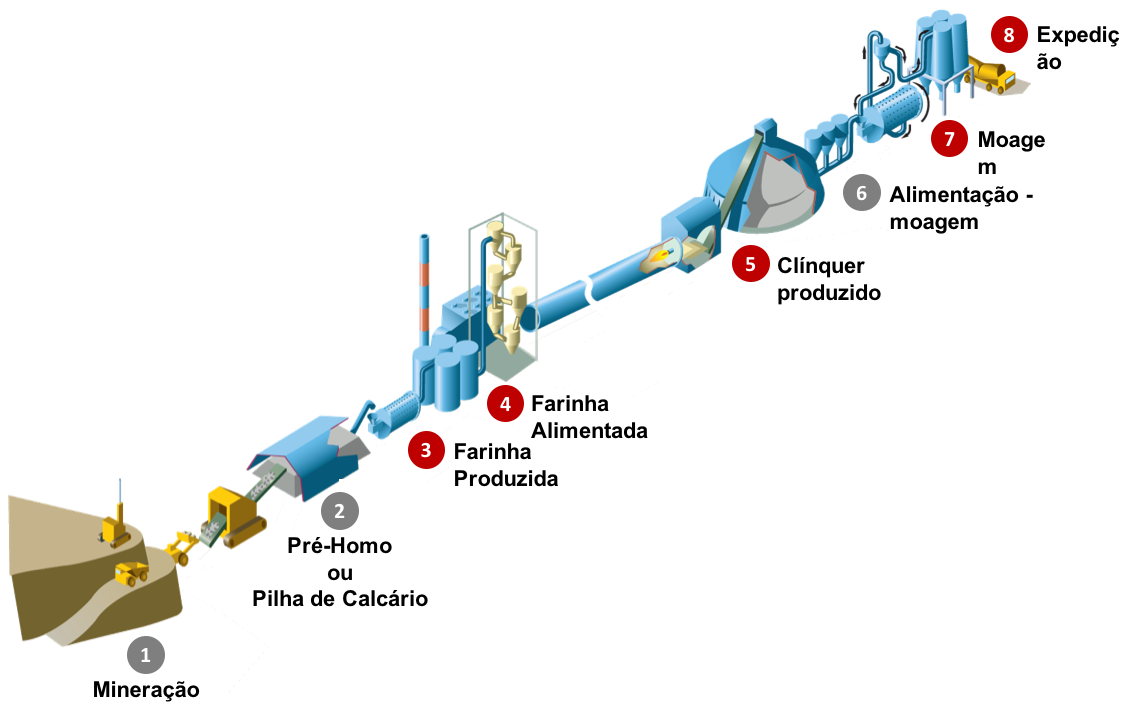
\includegraphics[scale=0.5]{cimento.png}
\caption{Representação das diversas etapas da produção de cimento}
\end{figure}
\end{frame}

\section{Análise dos Dados}

\begin{frame}
%%% plot com numero de entradas faltando nos dados 
\begin{figure}[H]
\centering
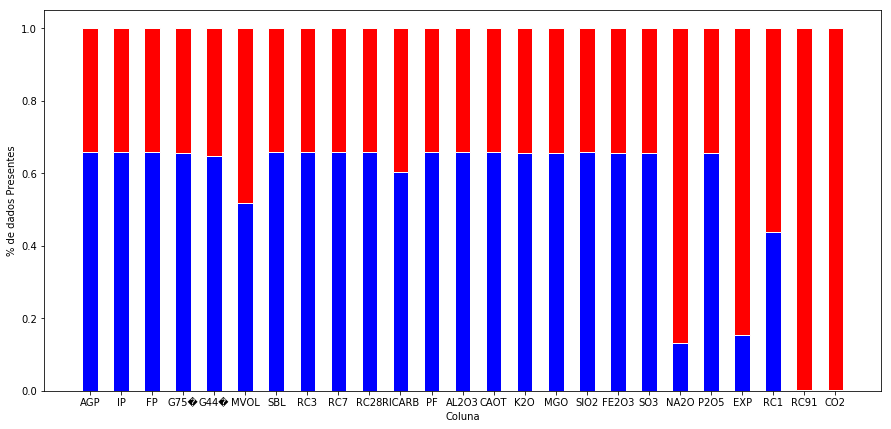
\includegraphics[scale=0.3]{slides_dados_pct}
\caption{Dados faltantes em cada coluna dos dados de Expedição de Cimento}
\end{figure}

\end{frame}

\begin{frame}
%%% slide apenas do RC3,RC7 e RC28
\begin{figure}[H]
\centering
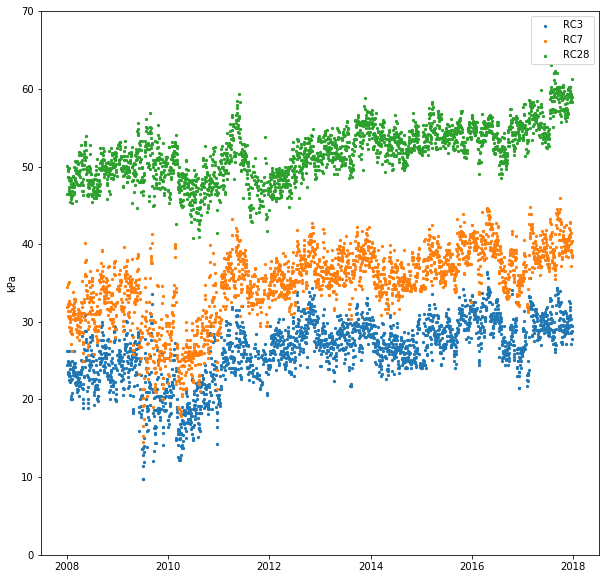
\includegraphics[scale=0.4]{slides_dados}
\caption{Dados que serão usados para o problema de Regressão}
\end{figure}

\end{frame}


\begin{frame}
%%% slide com tabela de correlação
\frametitle{Tabela de Correlação}
\begin{table}[H]
\centering
\begin{tabular}{l|lll}
\cline{2-4}
\textbf{}                  & \multicolumn{1}{l|}{RC3} & \multicolumn{1}{l|}{RC7} & \multicolumn{1}{l|}{RC28} \\ \hline
\multicolumn{1}{|l|}{RC3}  & 1                        & 0.734201                 & 0.388973                  \\ \cline{1-1}
\multicolumn{1}{|l|}{RC7}  & 0.734201                 & 1                        & 0.484725                  \\ \cline{1-1}
\multicolumn{1}{|l|}{RC28} & 0.388973                 & 0.484725                 & 1                         \\ \cline{1-1}
\end{tabular}
\caption{Correlação entre Índices de Resistência dos dados de
  Expedição de Cimento}
\label{corr3728}
\end{table}

\end{frame}

\begin{frame}
%%% slide com analise FFT só do RC28
\frametitle{Análise de Periodicidade}
\begin{figure}[H]
\centering
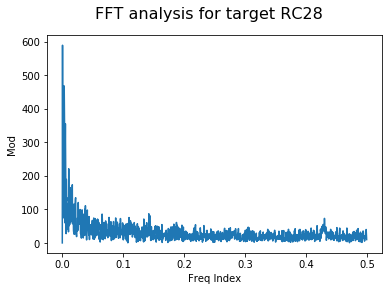
\includegraphics[scale=0.6]{FFT_RC28.png}
\caption{Análise Espectral para preditor RC28}
\end{figure}

\end{frame}


\begin{frame}
  \frametitle{Definição do Problema}
%%% slide definindo aprendizado supervisionado/regressao
  \begin{itemize}
    \item O problema de modelar o índice de Resistência é um problema de
  \textbf{Aprendizado Supervisionado} de \textbf{Regressão}.
    \item Queremos modelar uma função que aprenda com um conjunto de dados $\{(x_1,y_1)
\dots , (x_n,y_n)\}$ e possa nos gerar anotações inéditas $y^*$ para novas
entradas $x^*$.

    \item O aprendizado busca em uma certa família de funções aquela que maximiza a
      verossimilhança de uma distribuição implícita $p'(y | x)$ aprendida pelo modelo.
    
  \end{itemize}
  

  
\end{frame}

\begin{frame}
  \frametitle{Definição do Problema}

  \begin{itemize}
\item Em um primeiro momento podemos criar triplas de treino $(RC3_i,RC7_i,RC28_i)$, e queremos
  encontrar uma função: \\ 
  \begin{empheq}[box=\tcbhighmath]{align}
  \mathnormal{f}(RC3_i,RC7_i) = \widehat{RC28}_i 
  \end{empheq}
    \end{itemize}

Mas desse jeito o modelo não estaria usando nenhuma informação temporal dos dados.
    
\end{frame}


\begin{frame}
 
  \frametitle{Séries Temporais}

  \begin{itemize}
\item Dados anotados temporalmente, normalmente em intervalos regulares. O passado de
uma série pode trazer informação para prever o seu futuro.
\item Agora nosso problema
de aprendizado supervisionado leva em conta diversas anotações passadas. A
distribuição aprendida pelo modelo seria condicionada por diversas anotações
subsequentes passadas. 
  \begin{empheq}[box=\tcbhighmath]{align}
  p(y | x_{t} ,x_{t -1},x_{t -2},x_{t-3} , \dots, x_{t-T})
  \end{empheq}
\item Os dados da Intercement não estavam anotados em intervalos regulares,
  então eles foram reamostrados em intervalos de 1 dia. Com dias
  vazios sendo preenchidos com zeros.
    \end{itemize}
  
  %%% slide definindo serie temporal
\end{frame}

\section{Modelos Escolhidos}

\begin{frame}
%%% slide mostrando rede neural (mesmo diagrama da quali)
  \frametitle{Redes Neurais}
  \begin{empheq}[box=\tcbhighmath]{align}
    \mathnormal{f}_i (x)=  a_i = \sigma(W_i*a_{i-1} + b_i) 
  \end{empheq}

\begin{figure}
  \centering
  \def\layersep{2.5cm}

\begin{tikzpicture}[shorten >=1pt,->,draw=black!50, node distance=\layersep]
    \tikzstyle{every pin edge}=[<-,shorten <=1pt]
    \tikzstyle{neuron}=[circle,fill=black!25,minimum size=17pt,inner sep=0pt]
    \tikzstyle{input neuron}=[neuron, fill=green!50];
    \tikzstyle{output neuron}=[neuron, fill=red!50];
    \tikzstyle{hidden neuron}=[neuron, fill=blue!50];
    \tikzstyle{annot} = [text width=4em, text centered]

    % Draw the input layer nodes
    \foreach \name / \y in {1,...,4}
    % This is the same as writing \foreach \name / \y in {1/1,2/2,3/3,4/4}
    \node[input neuron, pin=left:Input \# RC3] (I-1) at (0,-1) {};
    \node[input neuron, pin=left:Input \# RC7] (I-2) at (0,-2) {};

    % Draw the hidden layer nodes
    \foreach \name / \y in {1,...,5}
        \path[yshift=0.5cm]
            node[hidden neuron] (H-\name) at (\layersep,-\y cm) {};

    % Draw the output layer node
    \node[output neuron,pin={[pin edge={->}]right:RC28}, right of=H-3] (O) {};

    % Connect every node in the input layer with every node in the
    % hidden layer.
    \foreach \source in {1,...,2}
        \foreach \dest in {1,...,5}
            \path (I-\source) edge (H-\dest);

    % Connect every node in the hidden layer with the output layer
    \foreach \source in {1,...,5}
        \path (H-\source) edge (O);

    % Annotate the layers
    \node[annot,above of=H-1, node distance=1cm] (hl) {Hidden layer};
    \node[annot,left of=hl] {Input layer};
    \node[annot,right of=hl] {Output layer};
\end{tikzpicture}
  \label{fig:nn}
\end{figure}


\end{frame}


\begin{frame}
\frametitle{Modelos Sequenciais: RNNs}
%%% slide definindo uma LSTM
\begin{figure}[H]
  
\scalebox{1}{
\begin{tikzpicture}[auto]

% RNN state cell =============================
\node[state] (h) {$\vect{h}$};
\node[op, below=30pt of h] (x) {$\vect{x}$};
\node[op, above=30pt of h] (yhat) {$\hat{\vect{y}}$};



% edges
\path[tedge] (x) edge node[below right= -4pt] {$\vect{U}$}  (h) ;
\path[tedge] (h) edge [out=-400,in=-320,looseness=8, distance=125pt] node[above right] {$\vect{W}$} (h);
\path[tedge] (h) edge node[below right = -4pt] {$\vect{V}$} (yhat);


\end{tikzpicture}
} % scalebox

  \caption{RNN genérica}
\end{figure}
\end{frame}

\begin{frame}
\frametitle{Modelos Sequenciais: RNNs}
%%% slide definindo uma LSTM 2
\begin{figure}[H]
  % RNN STATE CELL ====================================
\newcommand{\rnnSimple}[4]{

% operations
\node[state, minimum size=40pt,#4] (h#3) {$\vect{h}^{#1}$};
\node[op, minimum size=40pt,below=30pt of h#3] (x#3) {$\vect{x}^{#1}$};
\node[op, minimum size=40pt, above=30pt of h#3] (yhat#3) {$\hat{\vect{y}}^{#1}$};

% edges
\path[tedge] (x#3) edge node[below right= -4pt] {$\vect{U}$} (h#3);
\path[tedge] (h#3) edge node[below right = -4pt] {$\vect{V}$} (yhat#3);
}

\begin{figure}[H]
\hspace*{-1.0cm}
\scalebox{0.9}{
\begin{tikzpicture}[auto]

% timestep 1
\rnnSimple{(1)}{(0)}{t1}{}

% % timestep 0
\node[state, minimum size=40pt,left=50pt of ht1] (ht0) {$\vect{h}^{(0)}$};

% % timestep 2
\rnnSimple{(2)}{(1)}{t2}{right=50pt of ht1};


% % timestep 2
\rnnSimple{(3)}{(1)}{t3}{right=50pt of ht2};


% % state transfers
\path[tedge] (ht0) edge node[above right = 2pt] {$\vect{W}$} (ht1);
\path[tedge] (ht1) edge node[above right = 2pt] {$\vect{W}$} (ht2);
\path[tedge] (ht2) edge node[above right = 2pt] {$\vect{W}$} (ht3);

\end{tikzpicture}
}%\scalebox
\end{figure}

  \caption{RNN genérica através do tempo}
\end{figure}

\end{frame}


\begin{frame}
\frametitle{Modelos Sequenciais: LSTMs}
%%% slide definindo uma LSTM 2
  \resizebox{1\textwidth}{!}{
    

\begin{tikzpicture}[
    prod/.style={circle, draw, inner sep=0pt},
    ct/.style={circle, draw, inner sep=5pt, ultra thick, minimum width=10mm},
    ft/.style={circle, draw, minimum width=8mm, inner sep=1pt},
    filter/.style={circle, draw, minimum width=7mm, inner sep=1pt, path picture={\draw[thick, rounded corners] (path picture bounding box.center)--++(65:2mm)--++(0:1mm);
    \draw[thick, rounded corners] (path picture bounding box.center)--++(245:2mm)--++(180:1mm);}},
    mylabel/.style={font=\scriptsize\sffamily},
    >=LaTeX
    ]

\node[ct, label={[mylabel]Cell}] (ct) {$c_t$};
\node[filter, right=of ct] (int1) {};
\node[prod, right=of int1] (x1) {$\times$}; 
\node[right=of x1] (ht) {$h_t$};
\node[prod, left=of ct] (x2) {$\times$}; 
\node[filter, left=of x2] (int2) {};
\node[prod, below=5mm of ct] (x3) {$\times$}; 
\node[ft, below=5mm of x3, label={[mylabel]right:Forget Gate}] (ft) {$f_t$};
\node[ft, above=of x2, label={[mylabel]left:Input Gate}] (it) {$i_t$};
\node[ft, above=of x1, label={[mylabel]left:Output Gate}] (ot) {$o_t$};

\foreach \i/\j in {int2/x2, x2/ct, ct/int1, int1/x1,
            x1/ht, it/x2, ct/it, ct/ot, ot/x1, ft/x3}
    \draw[->] (\i)--(\j);

\draw[->] (ct) to[bend right=45] (ft);

\draw[->] (ct) to[bend right=30] (x3);
\draw[->] (x3) to[bend right=30] (ct);

\node[fit=(int2) (it) (ot) (ft), draw, inner sep=0pt] (fit) {};

\draw[<-] (fit.west|-int2) coordinate (aux)--++(180:7mm) node[left]{$x_t$};
\draw[<-] ([yshift=1mm]aux)--++(135:7mm);
\draw[<-] ([yshift=-1mm]aux)--++(-135:7mm);

\draw[<-] (fit.north-|it) coordinate (aux)--++(90:7mm) node[above]{$x_t$};
\draw[<-] ([xshift=1mm]aux)--++(45:7mm);
\draw[<-] ([xshift=-1mm]aux)--++(135:7mm);

\draw[<-] (fit.north-|ot) coordinate (aux)--++(90:7mm) node[above]{$x_t$};
\draw[<-] ([xshift=1mm]aux)--++(45:7mm);
\draw[<-] ([xshift=-1mm]aux)--++(135:7mm);

\draw[<-] (fit.south-|ft) coordinate (aux)--++(-90:7mm) node[below]{$x_t$};
\draw[<-] ([xshift=1mm]aux)--++(-45:7mm);
\draw[<-] ([xshift=-1mm]aux)--++(-135:7mm);
\end{tikzpicture}


%%% Local Variables:
%%% mode: latex
%%% TeX-master: '../quali'
%%% End:

    }

\end{frame}

\begin{frame}
\frametitle{Modelos Sequenciais: Encoder-Decoder}
%%% slide definindo uma LSTM 2
Redes Encoder-Decoder são modelos poderosos para criar \textit{representações}
de dados de entrada. A ideia é que esses modelos consigam gerar um vetor que
sumarize esses dados, e depois consiga reproduzi-los apenas sendo guiado por
esse vetor. A esse vetor se dá o nome de \textit{embedding}. 



\begin{figure}[H]
\centering
\begin{tikzpicture}[font=\sffamily]
\node[fill=brown!90!black, text=white, font=\sffamily\small, inner sep=2pt] (a) {\begin{tabular}{@{}r@{}}-0.2\\-0.1\\0.1\\0.4\\-0.3\\1.1\end{tabular}};

\node[fit=(a.north) (a.south), inner sep=1pt, right=1mm of a, minimum width=2cm, label=center:Decoder] (dec) {};
\node[fit=(a.north) (a.south), inner sep=1pt, left=1mm of a, minimum width=2cm, label=center:Encoder] (enc) {};

\begin{scope}[on background layer]
\fill[cyan!30] (dec.north west)--([yshift=5mm]dec.north east)--([yshift=-5mm]dec.south east)--(dec.south west)--cycle;
\fill[cyan!30] (enc.north east)--([yshift=5mm]enc.north west)--([yshift=-5mm]enc.south west)--(enc.south east)--cycle;
\end{scope}

\node[right=1mm of dec, fill=blue, single arrow] (b) {\phantom{a}};
\node[align=left, right=1mm of b] {Sequência de\\ saída};

\node[left=1mm of enc, fill=blue, single arrow] (c) {\phantom{a}};
\node[align=left, left=1mm of c] {Sequência de\\ entrada};
\end{tikzpicture}
%%% Local Variables:
%%% mode: latex
%%% TeX-master: t
%%% End:

\caption{ Diagrama de Rede Encoder-Decoder}

\end{figure}

\end{frame}

\begin{frame}
%%% slide com modelo Uber
\begin{figure}[H]
\centering
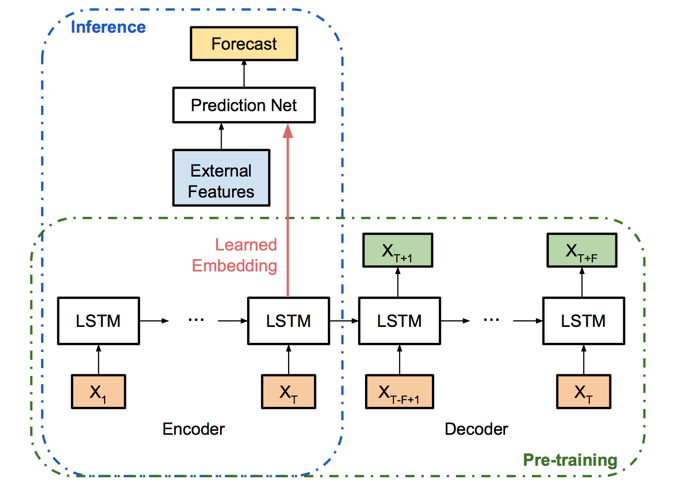
\includegraphics[scale=0.4]{uber.png}
\caption{Arquitetura do modelo Encoder-Decoder-Forecaster}
\end{figure}
\end{frame}

\begin{frame}
%%% slide inferencia bayesiana com a integral e os caralho
\end{frame}

\begin{frame}
  \frametitle{Dropout como Regularizador}
  \centering
%%% slide com dropout imagem da quali
  \resizebox{1\textwidth}{!}{
      



\begin{tikzpicture}

	\node[circle, draw, thick] (i1) {};
	\node[circle, draw, thick, above=2em of i1] (i2) {};
	\node[circle, draw, thick, above=2em of i2] (i3) {};
	\node[circle, draw, thick, below=2em of i1] (i4) {};
	\node[circle, draw, thick, below=2em of i4] (i5) {};
	
	\node[circle, draw, thick, right=4em of i1] (h1) {};
	\node[circle, draw, thick, right=4em of i2] (h2) {};
	\node[circle, draw, thick, right=4em of i3] (h3) {};
	\node[circle, draw, thick, right=4em of i4] (h4) {};
	\node[circle, draw, thick, right=4em of i5] (h5) {};
	
	\node[circle, draw, thick, right=4em of h1] (hh1) {};
	\node[circle, draw, thick, right=4em of h2] (hh2) {};
	\node[circle, draw, thick, right=4em of h3] (hh3) {};
	\node[circle, draw, thick, right=4em of h4] (hh4) {};
	\node[circle, draw, thick, right=4em of h5] (hh5) {};
	
	\node[circle, draw, thick, right=4em of hh2] (o1) {};
	\node[circle, draw, thick, right=4em of hh4] (o2) {};
	
	\draw[-stealth, thick] (i1) -- (h1);
	\draw[-stealth, thick] (i1) -- (h2);
	\draw[-stealth, thick] (i1) -- (h3);
	\draw[-stealth, thick] (i1) -- (h4);
	\draw[-stealth, thick] (i1) -- (h5);
	\draw[-stealth, thick] (i2) -- (h1);
	\draw[-stealth, thick] (i2) -- (h2);
	\draw[-stealth, thick] (i2) -- (h3);
	\draw[-stealth, thick] (i2) -- (h4);
	\draw[-stealth, thick] (i2) -- (h5);
	\draw[-stealth, thick] (i3) -- (h1);
	\draw[-stealth, thick] (i3) -- (h2);
	\draw[-stealth, thick] (i3) -- (h3);
	\draw[-stealth, thick] (i3) -- (h4);
	\draw[-stealth, thick] (i3) -- (h5);
	\draw[-stealth, thick] (i4) -- (h1);
	\draw[-stealth, thick] (i4) -- (h2);
	\draw[-stealth, thick] (i4) -- (h3);
	\draw[-stealth, thick] (i4) -- (h4);
	\draw[-stealth, thick] (i4) -- (h5);
	\draw[-stealth, thick] (i5) -- (h1);
	\draw[-stealth, thick] (i5) -- (h2);
	\draw[-stealth, thick] (i5) -- (h3);
	\draw[-stealth, thick] (i5) -- (h4);
	\draw[-stealth, thick] (i5) -- (h5);
	
	\draw[-stealth, thick] (h1) -- (hh1);
	\draw[-stealth, thick] (h1) -- (hh2);
	\draw[-stealth, thick] (h1) -- (hh3);
	\draw[-stealth, thick] (h1) -- (hh4);
	\draw[-stealth, thick] (h1) -- (hh5);
	\draw[-stealth, thick] (h2) -- (hh1);
	\draw[-stealth, thick] (h2) -- (hh2);
	\draw[-stealth, thick] (h2) -- (hh3);
	\draw[-stealth, thick] (h2) -- (hh4);
	\draw[-stealth, thick] (h2) -- (hh5);
	\draw[-stealth, thick] (h3) -- (hh1);
	\draw[-stealth, thick] (h3) -- (hh2);
	\draw[-stealth, thick] (h3) -- (hh3);
	\draw[-stealth, thick] (h3) -- (hh4);
	\draw[-stealth, thick] (h3) -- (hh5);
	\draw[-stealth, thick] (h4) -- (hh1);
	\draw[-stealth, thick] (h4) -- (hh2);
	\draw[-stealth, thick] (h4) -- (hh3);
	\draw[-stealth, thick] (h4) -- (hh4);
	\draw[-stealth, thick] (h4) -- (hh5);
	\draw[-stealth, thick] (h5) -- (hh1);
	\draw[-stealth, thick] (h5) -- (hh2);
	\draw[-stealth, thick] (h5) -- (hh3);
	\draw[-stealth, thick] (h5) -- (hh4);
	\draw[-stealth, thick] (h5) -- (hh5);
	
	
	\draw[-stealth, thick] (hh1) -- (o1);
	\draw[-stealth, thick] (hh1) -- (o2);
	\draw[-stealth, thick] (hh2) -- (o1);
	\draw[-stealth, thick] (hh2) -- (o2);
	\draw[-stealth, thick] (hh3) -- (o1);
	\draw[-stealth, thick] (hh3) -- (o2);
	\draw[-stealth, thick] (hh4) -- (o1);
	\draw[-stealth, thick] (hh4) -- (o2);
	\draw[-stealth, thick] (hh5) -- (o1);
	\draw[-stealth, thick] (hh5) -- (o2);
	
	\draw[-stealth, double, dashed, thick] (5.5,0) -- node[above] {dropout} (8.6, 0);
	
	
	%%% BOUNDARY %%%
	
	\node[circle, draw, thick, red, fill=red!10, right=15em of hh1] (i1) {};
	\node[circle, draw, thick, red, fill=red!10, above=2em of i1] (i2) {};
	\node[circle, draw, thick, above=2em of i2] (i3) {};
	\node[circle, draw, thick, below=2em of i1] (i4) {};
	\node[circle, draw, thick, below=2em of i4] (i5) {};
	
	\node[red] (icr) at (i1) {$\mathlarger{\mathlarger{\mathlarger{\mathlarger{\mathlarger{\bm{\times}}}}}}$};
	\node[red] (icr) at (i2) {$\mathlarger{\mathlarger{\mathlarger{\mathlarger{\mathlarger{\bm{\times}}}}}}$};
	
	\node[circle, draw, thick, red, fill=red!10, right=4em of i1] (h1) {};
	\node[circle, draw, thick, right=4em of i2] (h2) {};
	\node[circle, draw, thick, red, fill=red!10, right=4em of i3] (h3) {};
	\node[circle, draw, thick, red, fill=red!10, right=4em of i4] (h4) {};
	\node[circle, draw, thick, right=4em of i5] (h5) {};
	
	\node[red] (icr) at (h1) {$\mathlarger{\mathlarger{\mathlarger{\mathlarger{\mathlarger{\bm{\times}}}}}}$};
	\node[red] (icr) at (h3) {$\mathlarger{\mathlarger{\mathlarger{\mathlarger{\mathlarger{\bm{\times}}}}}}$};
	\node[red] (icr) at (h4) {$\mathlarger{\mathlarger{\mathlarger{\mathlarger{\mathlarger{\bm{\times}}}}}}$};
	
	\node[circle, draw, thick, right=4em of h1] (hh1) {};
	\node[circle, draw, thick, red, fill=red!10, right=4em of h2] (hh2) {};
	\node[circle, draw, thick, right=4em of h3] (hh3) {};
	\node[circle, draw, thick, red, fill=red!10, right=4em of h4] (hh4) {};
	\node[circle, draw, thick, right=4em of h5] (hh5) {};
	
	\node[red] (icr) at (hh2) {$\mathlarger{\mathlarger{\mathlarger{\mathlarger{\mathlarger{\bm{\times}}}}}}$};
	\node[red] (icr) at (hh4) {$\mathlarger{\mathlarger{\mathlarger{\mathlarger{\mathlarger{\bm{\times}}}}}}$};
	
	\node[circle, draw, thick, right=4em of hh2] (o1) {};
	\node[circle, draw, thick, right=4em of hh4] (o2) {};
	
	\draw[-stealth, thick] (i3) -- (h2);
	\draw[-stealth, thick] (i3) -- (h5);
	\draw[-stealth, thick] (i4) -- (h2);
	\draw[-stealth, thick] (i4) -- (h5);
	\draw[-stealth, thick] (i5) -- (h2);
	\draw[-stealth, thick] (i5) -- (h5);
	
	\draw[-stealth, thick] (h2) -- (hh1);
	\draw[-stealth, thick] (h2) -- (hh3);
	\draw[-stealth, thick] (h2) -- (hh5);
	\draw[-stealth, thick] (h5) -- (hh1);
	\draw[-stealth, thick] (h5) -- (hh3);
	\draw[-stealth, thick] (h5) -- (hh5);
	
	\draw[-stealth, thick] (hh1) -- (o1);
	\draw[-stealth, thick] (hh1) -- (o2);
	\draw[-stealth, thick] (hh3) -- (o1);
	\draw[-stealth, thick] (hh3) -- (o2);
	\draw[-stealth, thick] (hh5) -- (o1);
	\draw[-stealth, thick] (hh5) -- (o2);

\end{tikzpicture}


%%% Local Variables:
%%% mode: latex
%%% TeX-master: t
%%% End:

    }

    O Dropout força a rede neural a distribuir o aprendizado por todos os neurônios.
    
\end{frame}

\begin{frame}
  \frametitle{Dropout como Inferência Bayesiana}
  %%% slide com dropout imagem da quali

  É demonstrado que o Dropout pode ser interpretado como considerar uma
  distribuição de probabilidade em todos os parâmetros do modelo. Vamos usar
  como exemplo uma rede neural com uma camada oculta e dropout aplicado na
  camada de entrada, e na camada oculta. \\ 

  \begin{empheq}[box=\tcbhighmath]{align*}
  y^* &= \hat{a}W_2 \\
          &= (a * diag(\hat{\epsilon}_2))W_2 \\
          &=   \sigma(\hat{x}W_1 + b) *(diag(\hat{\epsilon}_2)W_2) \\
          &=   \sigma(x^* (diag(\hat{\epsilon}_1)W_1) + b) * (diag(\hat{\epsilon}_2)W_2) \\
  \end{empheq}

  
\end{frame}



\begin{frame}
  \frametitle{Dropout como Inferência Bayesiana}
  %%% slide com dropout imagem da quali
  Onde cada vetor $\epsilon_k$ é uma realização de um vetor de 0s e 1s seguindo
  uma distribuição de Bernoulli com probabilidade $p_k$ em cada posição: \\
  \begin{empheq}[box=\tcbhighmath]{align*}
    \hat{\epsilon}^{i}_k \sim Bernoulli(p_k)
  \end{empheq}
\end{frame}



\begin{frame}
  \frametitle{Dropout como Inferência Bayesiana}
  %%% slide com dropout imagem da quali
  Definindo-se: \\
  \begin{empheq}[box=\tcbhighmath]{align*}
    \hat{W_1} &:= diag(\hat{\epsilon}_1)W_1 \\
    \hat{W_2} &:= diag(\hat{\epsilon}_2)W_2
  \end{empheq}
Então podemos escrever a saída da rede neural como: \\
  \begin{empheq}[box=\tcbhighmath]{align*}
        y^*  =   \sigma(x \hat{W}_1 + b) * \hat{W}_2 =:
        \mathnormal{f}^{\hat{W}_1,\hat{W}_2,b}(x^*) \\
\end{empheq}
\end{frame}

\begin{frame}
  \frametitle{Dropout como Inferência Bayesiana}
  %%% slide com dropout imagem da quali

  Dessa maneira, podemos estimar os dois primeiros momentos das predições de
  maneira simples: \\
  
  \begin{empheq}[box=\tcbhighmath]{align*}
   \widetilde{\mathbb{E}}[y^*] &= \frac{1}{B}\sum^B_{B=1}\hat{y}^*_{(B)} \\ 
   \widetilde{\mathit{Var}}[y^*]  &= \frac{1}{B}\sum^B_{B=1}(\hat{y}^*_{(B)} - \bar{y}^*)^2 
  \end{empheq}

\end{frame}


\begin{frame}
%%% slide do modelo da uber com zoom
\end{frame}

\begin{frame}
%%% formulas de variancia no modelo uber

  Finalmente, estimamos a incerteza do modelo usando o MC Dropout. E o ruído
  inerente usando a variância amostral de um conjunto de dados de validação:\\ 

  \begin{empheq}[box=\tcbhighmath]{align*}
   \widetilde{\mathit{Var}}[f^W(x^*)]  &=
   \frac{1}{B}\sum^B_{B=1}(\hat{y}^*_{(B)} - \hat{y}^*)^2 \\ 
   \widetilde{\sigma}^2 &= \frac{1}{V}\sum^V_{V=1}(y'_v - f^W(x'_v))^2 
  \end{empheq}

\end{frame}

\section{Resultados}

\begin{frame}
  %%% Divisão do dataset
  \frametitle{Preparo dos Dados}
  \begin{itemize}
    \item Dados foram divididos entre \textbf{treino} e \textbf{validação}.
      Usamos os dados anotados de 2008 até 2015 para treinar os modelos e de
      2016 em diante para valida-los, testando a sua capacidade de
      generalização.
      
    \item Todos os dados foram transformados segundo a equação $\textbf{z} =
      \frac{\textbf{x} - \mu}{\sigma}$, para que ficassem com média 0 e
      variância unitária. Isso evitou efeitos indejados no treinamento dos modelos.
      
    \end{itemize}
    \begin{figure}[H]
  \centering
  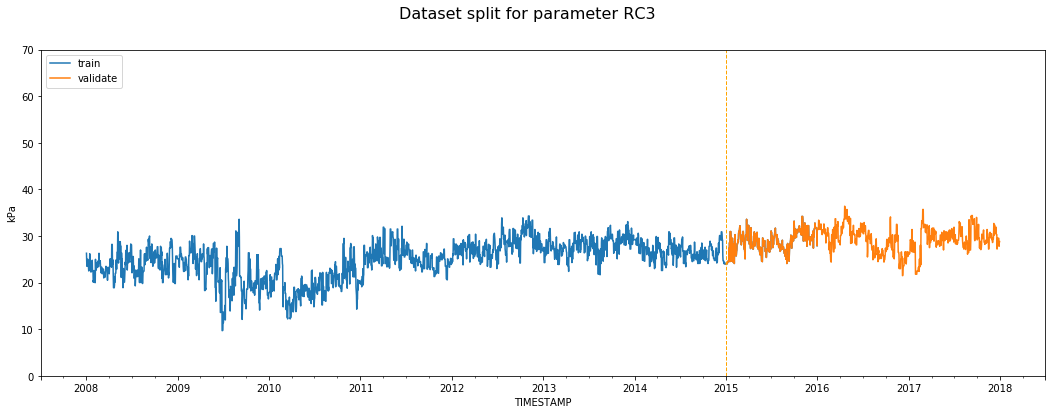
\includegraphics[width=0.9\columnwidth]{split_2008-2015-2017RC3.png}
\end{figure}

\end{frame}


\begin{frame}
%%% resultados modelos não-sequenciais
\end{frame}


\begin{frame}
%%% preparacao dos dados para modelos de sequencia
\end{frame}

\begin{frame}
%%% resultados modelo uber
\end{frame}

\begin{frame}
%%% conclusão até agora
\end{frame}

\begin{frame}
%%% direção futura imagem do cronograma
\end{frame}















\end{document}